%%%%%%%%%%%%%%%%%%%%%%%%%%%%%%%%%%%%%%%%%%%%%%%%%%%%%%%%%%%%%%%%%%%
\section{Étape 4: Sélectionner la plateforme adaptée} \label{sec:methodo_step4}
%%%%%%%%%%%%%%%%%%%%%%%%%%%%%%%%%%%%%%%%%%%%%%%%%%%%%%%%%%%%%%%%%%%


    Les deux premières étapes ont permis de trouver et de caractériser de potentielles architectures. À l'aide de plusieurs benchmarks, certaines caractéristiques clés des architectures ont pu être obtenues. Lors de l'étape 3, l'extraction et la modélisation des \glspl{hotspot} ont été faites.  Cette quatrième étape consiste à réaliser le choix de l'architecture la plus adaptée pour l'exécution de chaque hot spot. Ce choix est réalisé en prenant en considération la performance des architectures, les besoins de l'application étudiée ainsi que d'autres critères (voir \autoref{pic:methodo_step4}).
    
    \begin{figure}
        \center
        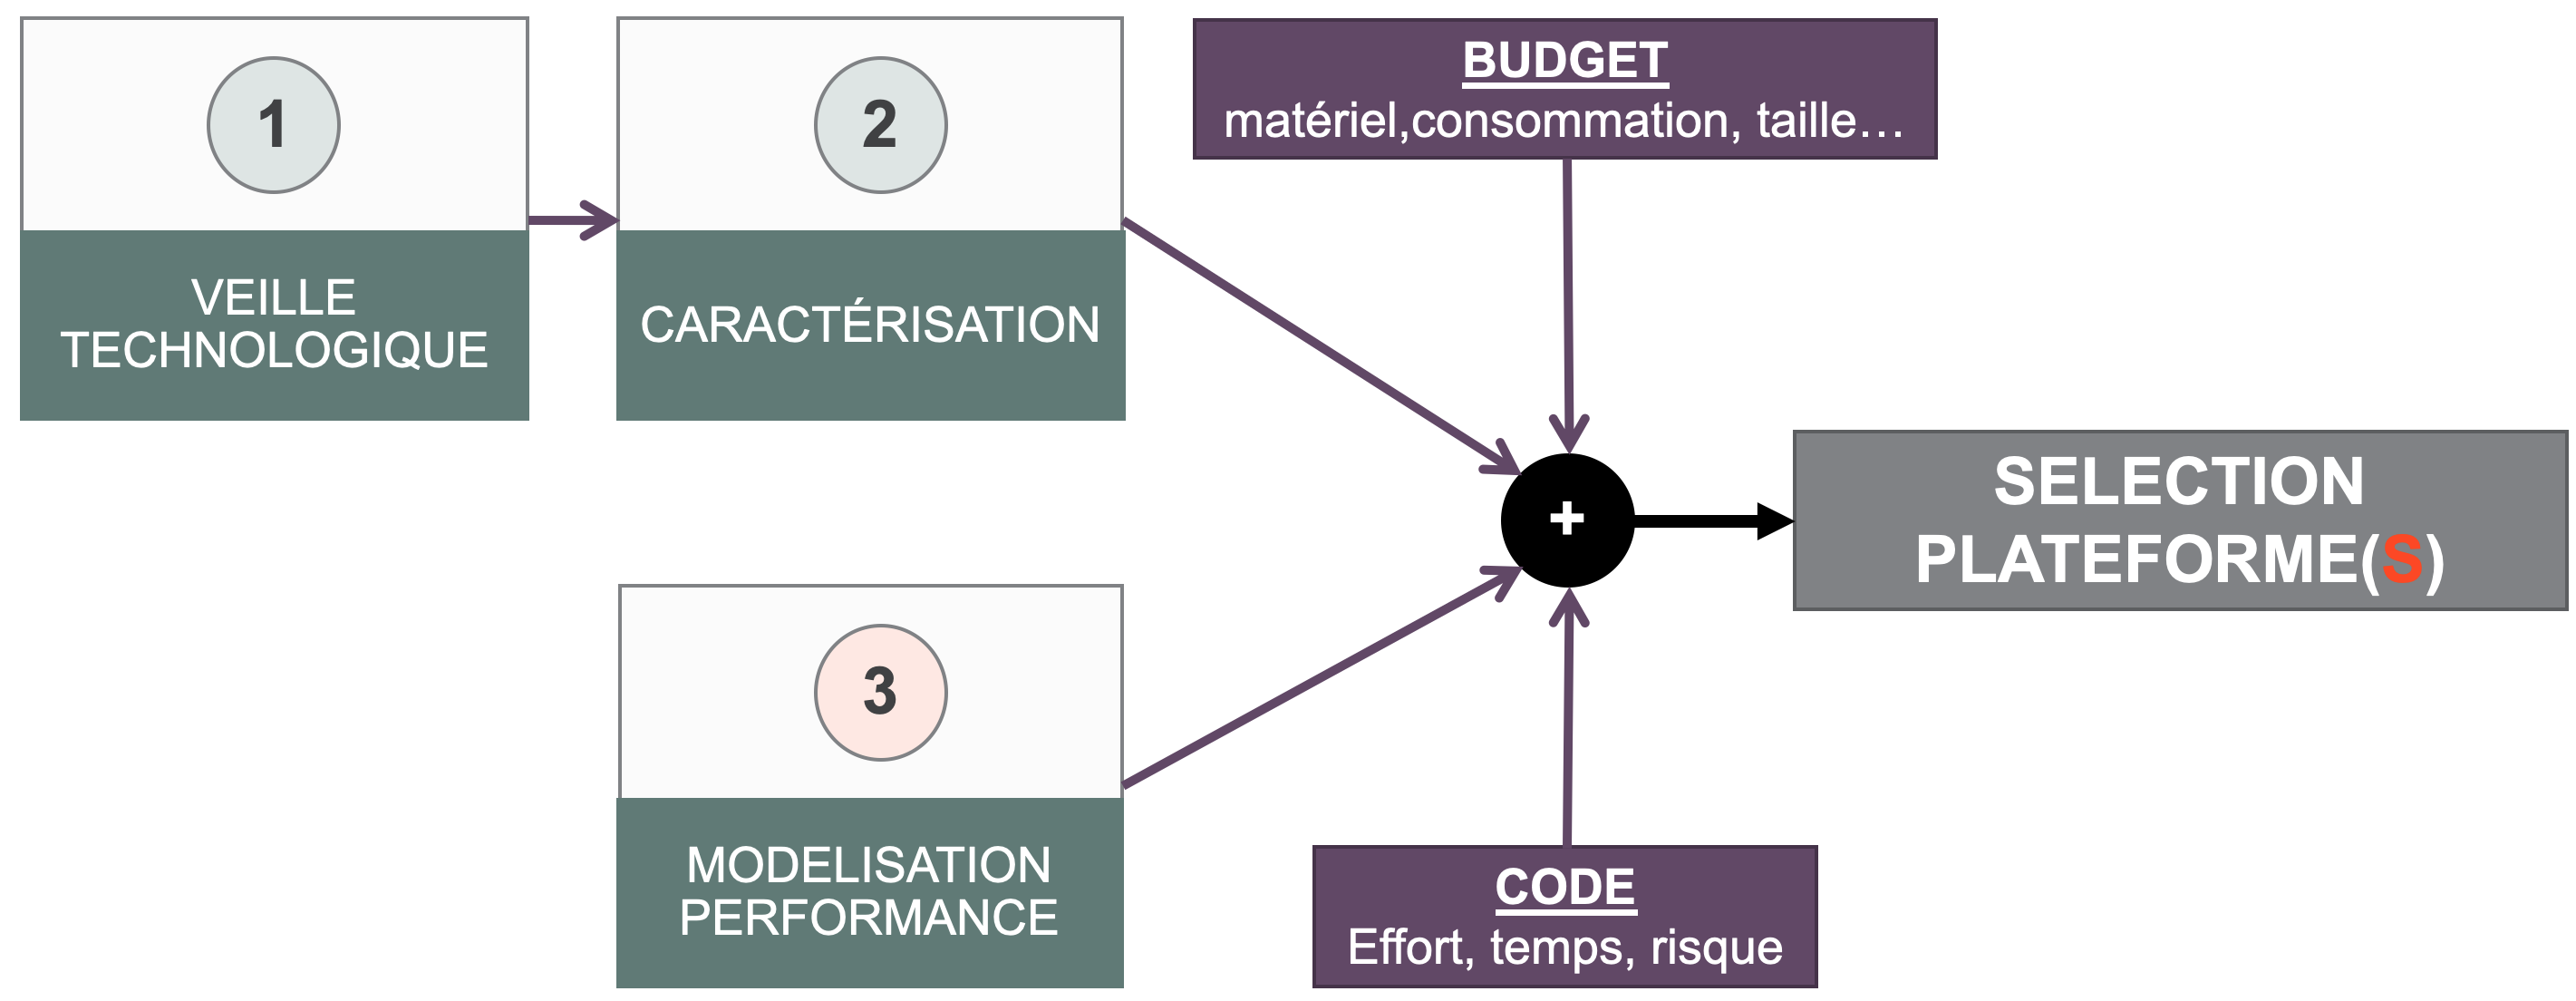
\includegraphics[width=14cm]{images/methodo_step4.png}
        \caption{\label{pic:methodo_step4}L'étape 4 consiste à choisir les plateformes adaptées aux différents noyaux en fonction de plusieurs critères.}
    \end{figure}



%%%%%%%%%%%%%%%%%
\subsection{Le coût}
%%%%%%%%%%%%%%%%%
    
   Le prix des architectures est un élément important pour choisir la ou les architectures utilisées pour la construction de la plateforme. Cependant, utiliser le prix unitaire des accélérateurs choisis n'est pas suffisant et il est nécessaire de prendre en compte d'autres paramètres dans le calcul du prix appelé coût total de possession (TCO). Il prend en compte tous les coûts engendrés par le centre de données durant son cycle de vie: construction des bâtiments, consommation électrique, etc.
   %Le budget pour la construction du premier centre exascale européen est de 500 millions d'euros \cite{SergiGirona2018}.
    
    \paragraph{Le prix du matériel} 
        Le  prix des accélérateurs et du matériel nécessaires à la construction du supercalculateur constituent une part significative dans le calcul du coût. En fonction du prix de l'accélérateur, une solution moins performante pourra lui être préférée. Les cartes FPGA sont un bon exemple d'architectures très performantes, mais peu utilisées dans les supercalculateurs. Bien que la complexité de programmation y participe, le prix des cartes FPGA est une raison majeure de leur faible utilisation dans les plateformes modernes.
    
    \paragraph{La consommation électrique}
        La consommation électrique de la plateforme finale est devenue un critère très important dans le choix du matériel. La consommation des centres de données est un réel investissement qui doit être mesuré et anticipé lors de l'achat du matériel. Un supercalculateur consommant 10 MW engendrera une facture de plusieurs millions d'euros chaque année. Le prix de l'électricité et l'enveloppe énergétique disponible pour le calcul varient avec l'emplacement choisi pour installer le centre de calcul. La majorité des centres ayant des lignes électriques déjà construites ne peuvent acheminer qu'une quantité limitée de courant. L'enveloppe énergétique disponible est alors une contrainte forte pouvant favoriser l'utilisation d'une architecture plus efficace énergétiquement.
        
        En comparant  l'intensité opérationnelle d'un kernel (\gls{oikernel}) et l'équilibre arithmétique de l'architecture (\gls{equilibrearchi}) il est possible d'estimer la pertinence d'un accélérateur pour un noyau. Des valeurs proches indiquent que l'architecture ciblée est adaptée au code étudié et que l'accélérateur choisi aura un meilleur rendement énergétique. Un code faisant peu de calculs flottants ne nécessitera pas l'utilisation de coeurs complexes réalisant plusieurs dizaines de \gls{FLOP} par cycle. Bien que non utilisés, ces composants impactent le prix de la solution, mais aussi sa consommation électrique. 
        
                %La chaleur de la zone géographique de son installation impactant le refroidissement nécessaire. Ainsi en 2018, Microsoft a décidé de couler ses serveurs au fond de l'océan pour profiter d'un refroidissement gratuit \cite{ChristineHall2018}.
            
    \paragraph{La taille du centre de données} 
        Souvent les centres de données sont déjà existants et la taille disponible pour la création d'un supercalculateur ou l'ajout de nouveaux serveurs est une contrainte forte. Certaines solutions prenant plus ou moins de place pour être installées, le ratio $\frac{flop}{m^2}$ peut alors être calculé pour évaluer la densité des serveurs pour s'adapter aux contraintes du lieu. Si le bâtiment doit être construit pour accueillir le supercalculateur, son coût doit entrer dans le calcul de la solution finale.




%%%%%%%%%%%%%%%%%
\subsection{La performance}
%%%%%%%%%%%%%%% \cite{Rodero2012}%%
    D'autres critères concernant la performance et l'optimisation du code doivent être pris en compte pour choisir la ou les architectures utilisées pour accélérer l'exécution de l'application.
    
    \paragraph{Performance du noyau}
        Bien sûr, le gain de performance obtenu après le portage d'un \gls{kernel} sur un accélérateur est un critère important.
        La performance du noyau a un impact financier, car s'il est exécuté plus rapidement, d'autres applications pourront alors accéder à la plateforme. Les clients de supercalculateurs ont généralement un budget fixe et de multiples applications à exécuter. Ils cherchent alors à optimiser l'utilisation des ressources informatiques par les différents codes. Bien que l'on considère qu'il est nécessaire de porter individuellement chaque noyau sur l'accélérateur le plus adapté, il faut aussi prendre en considération le reste de l'application, mais aussi les applications des autres utilisateurs. Si une seule des applications ne bénéficie pas des performances d'un accélérateur, il serait plus pertinent d'opter pour un accélérateur adapté à plusieurs applications exécutées sur la plateforme. 
    
     
    \paragraph{Difficulté du portage}
        Les transformations de codes nécessaires pour porter le code d'un kernel sur une architecture doivent être évaluées. Celles-ci peuvent avoir un impact sur les performances finales (incapacité à réaliser les optimisations nécessaires) ou sur le coût (recours à des programmeurs expérimentés).  Suivant l'architecture choisie, il faudra peut-être coder l'application avec un nouveau langage, utiliser de nouvelles librairies ou de nouveaux modèles de programmation. Lorsque l'implémentation d'une optimisation est décidée, le risque de ne pas parvenir à obtenir les performances espérées doit lui aussi être mesuré. Le temps optimal, noté \gls{tempsoptimal}, pour exécuter l'application considère que l'application utilise de façon optimale l'architecture. Cependant pour atteindre ces performances, le noyau peut nécessiter l’utilisation d'optimisations complexes, pouvant être difficile à implémenter sur des applications industrielles. Il peut arriver qu'une optimisation moins performante soit préférée, car la transformation du code est plus facile. Le temps et le nombre de programmeurs nécessaires à son implémentation entrent alors aussi en considération dans le prix de la solution.
    
                           